
\documentclass[a4paper,12pt]{article} % добавить leqno в [] для нумерации слева

\usepackage[left=2cm,right=2cm,
top=2cm,bottom=2cm,bindingoffset=0cm]{geometry}


\usepackage{cmap}

\usepackage{amsmath,amsfonts,amssymb,amsthm,mathtools} % AMS
\usepackage{mathtext}
\usepackage[TS1,T2A]{fontenc}
\usepackage[utf8]{inputenc}
\usepackage{siunitx}

\usepackage[english,russian]{babel}

\usepackage{fontspec}         % пакет для подгрузки шрифтов

\setmainfont{Times New Roman}       % задаёт основной шрифт документа


\usepackage{icomma} 
\mathtoolsset{showonlyrefs=true} % Показывать номера только у тех формул, на которые есть \eqref{} в тексте.
\usepackage{euscript}	 % Шрифт Евклид
\usepackage{mathrsfs} % Красивый матшрифт
\usepackage{enumitem}
\usepackage{tikz} % To generate the plot from csv
\usepackage{pgfplots}

\usepackage{multicol}
\setlength{\columnsep}{1cm}

%\renewcommand{\theenumi}{(\Asbuk{enumi})}
%\renewcommand{\labelenumi}{\Asbuk{enumi})}

\makeatletter
\AddEnumerateCounter{\asbuk}{\russian@alph}{щ}
\makeatother

%%% Заголовок
\author{Касьянова Ксения, Федорчук Яна (ЭО-15-01) }
\title{Домашнее задание 2}
\date{\today}


\begin{document}

\maketitle

\subsubsection*{(а)}	

Сравним средние уровни инфляции в таргетирующих её странах:  до инфляционного таргетирования $ \bar{X}_{pre} = 10.9 $ и после инфляционного таргетирования $ \bar{X}_{post} = 5.09$. 

Проведем парный t-тест: $ t = 3.355, p-value = 0.002294$

Значение $ p-value < 0.05 $ говорит о том, что разница в средних $ \Delta \bar{X} = 5.8 $  статистически значима.    

Несмотря на это мы знаем, что на снижение инфляции могли оказать влияние  общие тренды в экономике, а вовсе не переход стран к таргетированию инфляции, поэтому  на основе
этого результата сделать вывод о воздействии инфляционного
таргетирования на уровень инфляции нельзя.

	
\begin{figure}[h!]
	\centering
	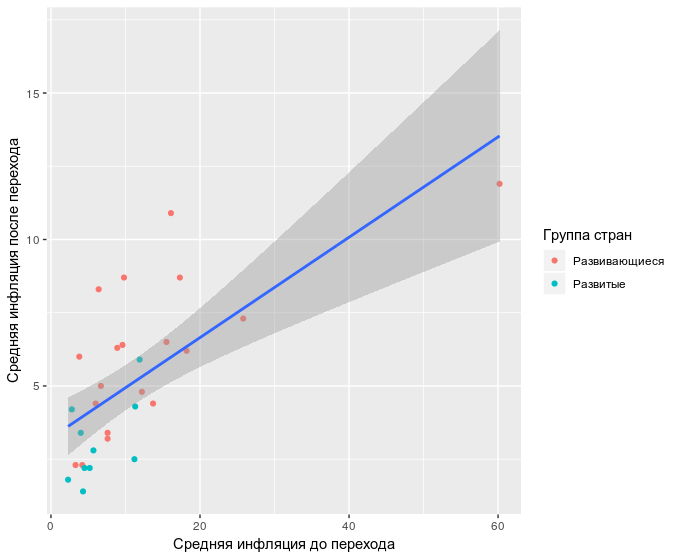
\includegraphics[width=0.7\linewidth]{Rplot}
	\caption[Диаграмма рассеяния]{Диаграмма рассеяния}
	\label{fig:rplot1}
\end{figure}



\newpage


	
	
\subsubsection*{(б)}	

Оценим регрессию разницы уровней инфляции до и после инфляционного таргетирования по дамми, которая равна 1, если страна таргетирует инфляцию.


Для полной выборки стран:

\begin{table}[h!]
	\centering
	\begin{tabular}{rrrrr}
		\hline
		& Estimate & Std. Error & t value & Pr(>|t|) \\ 
		\hline
		(Intercept) & -0.2362 & 0.9807 & -0.24 & 0.8101 \\ 
		$ D $ & -5.5707 & 2.1081 & -2.64 & 0.0092 \\ 
		\hline
	\end{tabular}
\end{table}

,
Для выборки развивающихся стран:

\begin{table}[h!]
	\centering
	\begin{tabular}{rrrrr}
		\hline
		& Estimate & Std. Error & t value & Pr(>|t|) \\ 
		\hline
		(Intercept) & -2.2727 & 0.5766 & -3.94 & 0.0004 \\ 
		$ D $ & -0.9773 & 1.0315 & -0.95 & 0.3510 \\ 
		\hline
		\end{tabular}
		\end{table}


Для выборки развитых стран:

\begin{table}[h!]
	\centering
	\begin{tabular}{rrrrr}
		\hline
		& Estimate & Std. Error & t value & Pr(>|t|) \\ 
		\hline
		(Intercept) & 0.3036 & 1.2465 & 0.24 & 0.8081 \\ 
		$ D $ & -7.4562 & 2.8881 & -2.58 & 0.0113 \\ 
		\hline
		\end{tabular}
		\end{table}
	
	
	
Как мы видим по таблице, для выборки всех стран коэффициент при дамми-переменной значим на 1\% уровне.
Такой результат говорит о  положительном воздействии перехода к инфляционному таргетированию на уровень инфляции. 


Для выборки развитых стран коэффициент при дамми-переменной значим на 5\% уровне, а для  выборки развивающихся стран не значим. Опираясь на полученные оценки параметров, можно сделать вывод, что положительное влияние инфляционного таргетирования наблюдается только для развитых стран.



\subsubsection*{(в)}	

Оценим регрессию разницы уровней инфляции до и после инфляционного таргетирования по дамми, которая равна 1, если страна таргетирует инфляцию, и контрольной перменной  $ X_pre $ значению инфляции до таргетирования (для контроля на наличие регрессии к среднему значению).
 
Для полной выборки стран:
 
\begin{table}[h!]
	\centering
	\begin{tabular}{rrrrr}
		\hline
		& Estimate & Std. Error & t value & Pr(>|t|) \\ 
		\hline
		(Intercept) & 4.7618 & 0.3619 & 13.16 & < 0.0001 \\ 
		$ D $ & -1.2539 & 0.7164 & -1.75 & 0.0824 \\ 
		$ X_{pre} $ & -0.8546 & 0.0263 & -32.45 & < 0.0001 \\ 
		\hline
	\end{tabular}
\end{table}

Для выборки развивающихся стран:

\begin{table}[h!]
	\centering
	\begin{tabular}{rrrrr}
		\hline
		& Estimate & Std. Error & t value & Pr(>|t|) \\ 
		\hline
		(Intercept) & 0.8521 & 0.3672 & 2.32 & 0.0275 \\ 
		$ D $ & 0.3088 & 0.4574 & 0.68 & 0.5049 \\ 
		$ X_{pre} $ & -0.6979 & 0.0605 & -11.54 & < 0.0001 \\ 
		\hline
	\end{tabular}
\end{table}

\newpage

Для выборки развитых стран:

\begin{table}[h!]
	\centering
	\begin{tabular}{rrrrr}
		\hline
		& Estimate & Std. Error & t value & Pr(>|t|) \\ 
		\hline
		(Intercept) & 5.7226 & 0.4033 & 14.19 & < 0.0001 \\ 
		$ D $ & -1.2640 & 0.8717 & -1.45 & 0.1502 \\ 
		$ X_{pre} $  & -0.8723 & 0.0269 & -32.46 & < 0.0001 \\ 
		\hline
	\end{tabular}
\end{table}

Для всех трех выборок после включения контрольной переменной мы наблюдаем следующее: 
коэффициент при дамми становится незначительным, а коэффициент при уровне инфляции до таргетирования значим на 1\% уровне. 


Также отметим изменения в $ R^2:  $ 
от $ 0.05 $  до $ 0.89 $ для всех стран, от $ 0.03 $ до $ 0.82 $ для развивающихся стран и от $ 0.06 $ до $ 0.91 $ для развитых стран. 


Такие результаты говорят нам о наличии регрессии к среднему значению, что  отражает тот факт, что если во всех странах  изначально наблюдались высокие показатели инфляции (выше среднего), то они  
могли уменьшиться в следующем периоде частично из-за статистической вероятности оказаться ближе к среднему значению. То есть показатели инфляции изменились бы даже без таргетинга. 



Для развитых стран мы видим положительное влияние в обоих случаях (коэффициент при дамми меньше 0). 
Для развивающихся стран коэффициент при дамми без контроля меньше 0, а с контролем больше 0. 
Это может объясняться тем фактом, что
переход на таргетинг был наиболее привлекательным для стран с изначально завшенными показателями инфляции в случае с развивающимися странами. 
То есть  использование политики ИТ 
позволило странам снизить инфляцию до низких уровней и уменьшить волатильность в случае с развитыми странами, при 
этом таргетирующие страны смогли догнать 
нетаргетирующие по некоторым показателям по причинам не  свзанным с самим  таргетингом в случае с развивающимися странами.













\end{document}